% Style based on 'Leap Day' by Matt Graham:
%
%   https://github.com/mattgraham/Leap-Day
%
\documentclass{article}
\usepackage[a0paper]{geometry}
\usepackage{etoolbox}
\usepackage{xcolor}
\usepackage{graphicx}
%\usepackage{fontawesome}
\usepackage{tikz}
\usetikzlibrary{calc}
\usetikzlibrary{fadings}
\usepackage[hidelinks]{hyperref}

% fonts

\usepackage{lmodern}
\usepackage[T1]{fontenc}

% Fix small math symbols.
% source: http://tex.stackexchange.com/questions/74623/big-integral-in-lmodern
% TODO: Is there a better way to fix this?
\DeclareFontFamily{OMX}{lmex}{}
\DeclareFontShape{OMX}{lmex}{m}{n}{<-> lmex10}{}

\sffamily
\renewcommand{\familydefault}{\sfdefault}

\renewcommand{\tiny}        {\fontsize{ 20.74pt}{ 25pt}\selectfont}
\renewcommand{\scriptsize}  {\fontsize{ 24.88pt}{ 30pt}\selectfont}
\renewcommand{\footnotesize}{\fontsize{ 29.86pt}{ 37pt}\selectfont}
\renewcommand{\small}       {\fontsize{ 35.83pt}{ 45pt}\selectfont}
\renewcommand{\normalsize}  {\fontsize{ 43.00pt}{ 54pt}\selectfont}
\renewcommand{\large}       {\fontsize{ 51.60pt}{ 64pt}\selectfont}
\renewcommand{\Large}       {\fontsize{ 61.92pt}{ 77pt}\selectfont}
\renewcommand{\LARGE}       {\fontsize{ 74.30pt}{ 93pt}\selectfont}
\renewcommand{\huge}        {\fontsize{ 89.16pt}{112pt}\selectfont}
\renewcommand{\Huge}        {\fontsize{107.00pt}{134pt}\selectfont}

\normalsize

% spaces

\setlength\parindent      { 2em}
\setlength\parskip        { 0pt plus .5ex}
\setlength\floatsep       {45pt plus  5pt minus  5pt}
\setlength\textfloatsep   {86pt plus  9pt minus 18pt}
\setlength\intextsep      {45pt plus  5pt minus 15pt}
\setlength\dblfloatsep    {45pt plus  5pt minus  5pt}
\setlength\dbltextfloatsep{86pt plus  9pt minus 18pt}

\setlength\abovedisplayskip     {32pt plus 3pt minus 3pt}
\setlength\abovedisplayshortskip{14pt plus 3pt minus 3pt}
\setlength\belowdisplayskip     {\abovedisplayskip}
\setlength\belowdisplayshortskip{\abovedisplayskip}

% list environments

\setlength\leftmargini  {2em}
\leftmargin  \leftmargini
\setlength\leftmarginii  {2.2em}
\setlength\leftmarginiii {1.87em}
\setlength\leftmarginiv  {1.7em}
\setlength\leftmarginv  {.5em}
\setlength\leftmarginvi {.5em}
\setlength  \labelsep  {.5em}
\setlength  \labelwidth{\leftmargini}
\addtolength\labelwidth{-\labelsep}
\makeatletter
\@beginparpenalty -\@lowpenalty
\@endparpenalty   -\@lowpenalty
\@itempenalty     -\@lowpenalty
\makeatother
\renewcommand\labelitemi{{\fontfamily{lmr}\selectfont\textbullet}}
\renewcommand\labelitemii{\normalfont\bfseries \textendash}
\renewcommand\labelitemiii{\textasteriskcentered}
\renewcommand\labelitemiv{\textperiodcentered}

% style lengths

\def\setnewlength#1#2{%
  \newlength{#1}%
  \deflength{#1}{#2}}

\setnewlength\safetymargin{3cm}
\setnewlength\headerheight{.2\paperwidth}
\setnewlength\headeryellowbarheight{.065\paperwidth}
\setnewlength\headeryellowbarlength{.8\paperwidth}
\setnewlength\footerheight{.1\paperwidth}
\setnewlength\footercontentheight{.6\footerheight}
\setnewlength\photobarheight{.128\paperwidth}
\setnewlength\photomargin{.01\paperwidth}
\setnewlength\photobarbottommargin{.03\paperwidth}
\setnewlength\textboxinnermargin{1em}

% style colors

\definecolor{LDbackground}{HTML}{CECACA}
\definecolor{LDblue}{cmyk}{1,0,0,0}
\definecolor{LDyellow}{HTML}{FFCC00}
\definecolor{LDyellowborder}{HTML}{F0B500}
\definecolor{LDtextborder}{HTML}{CBCBCB}
\pagecolor{LDbackground}

% textbox

\def\textbox(#1) at (#2) [#3] <#4> #5{%
  \def\textboxname{#1}%
  \def\textboxpos{#2}%
  \def\textboxalign{#3}%
  \def\textboxwidth{#4}%
  \def\textboxtitle{#5}%
  \node[fill=white,draw=LDtextborder,inner sep=\textboxinnermargin,shift={(0,-2\textboxinnermargin)},rounded corners=.5ex] (contents #1) at (#2) [#3] \bgroup%
    \begin{minipage}{#4}}%
\def\endtextbox{%
    \end{minipage}%
  \egroup;%
  \node[black,inner sep=0pt,shift={(\textboxinnermargin,0.65em)}] at (contents \textboxname.north west) [above right] {%
    \large\sffamily\bfseries\textboxtitle};
}

% QR code

\ifx\directlua\undefined
  \def\qrcode<#1>[#2]#2{%
    \errmessage{qrcode: Please compile with `lualatex`.}}
\else
  \directlua{qrcode=dofile(kpse.find_file("qrcodehelper.lua"))}
  \def\hrefwrapper#1#2{% clickable link, only if `hyperref` package is loaded
    \ifcsdef{href}{%
      \href{#1}{#2}}{%
      #2}}
  \def\qrcode<#1>[#2]#3{%
    \bgroup%
      \newlength{\qrsize}%
      \setlength{\qrsize}{#1}%
      \def\qrcodecolor{#2}%
      \hrefwrapper{#3}{\directlua{qrcode.generate("\luaescapestring{#3}")}}%
    \egroup}
\fi

% misc

\renewcommand{\emph}[1]{%
  {\color{LDblue}#1}}

\pagestyle{empty}

\begin{document}%
\begin{tikzpicture}[remember picture,overlay,line width=.001\paperwidth]

% header

\fill[color=LDblue] ($(current page.north west)+(-\safetymargin,+\safetymargin)$) rectangle ($(current page.north east)+(+\safetymargin,-\headerheight)$);
\draw[color=LDyellowborder,fill=LDyellow,rounded corners=.5ex] ($(current page.north west)+(-\safetymargin,-\headerheight+.5\headeryellowbarheight)$) rectangle ($(current page.north west)+(\headeryellowbarlength,-\headerheight-.5\headeryellowbarheight)$);
\node[color=white] at ($(current page.north)-(0,.4\headerheight)$) {%
  \sffamily\bfseries\fontsize{100}{100}\selectfont%
  SIAM Student Chapter Delft};%
\node[color=white] at ($(current page.north)-(0,.65\headerheight)$) {%
  \sffamily\fontsize{60}{60}\selectfont%
  Delft University of Technology};
\node[color=black,right,inner sep=0pt] at ($(current page.north west)+(3cm+\textboxinnermargin,-\headerheight)$) {%
  \sffamily\fontsize{45}{45}\selectfont%
  \textbf{Visit our homepage:} \quad \href{http://sscdelft.github.io}{http://sscdelft.github.io}};

% footer

\setnewlength{\footervmargin}{.5\footerheight-.5\footercontentheight}
\setnewlength{\footerhmargin}{\footervmargin}


\draw[color=LDtextborder,fill=LDblue] ($(current page.south west)+(-\safetymargin,-\safetymargin)$) rectangle ($(current page.south east)+(\safetymargin,\footerheight)$);
\node [left,inner sep=0pt] at ($(current page.south east)+(-\footerhmargin,.5\footerheight)$) {
  \qrcode<\footercontentheight>[white]{http://sscdelft.github.io}};
\node [left,inner sep=0pt,white] at ($(current page.south east)+(-\footerhmargin-\footervmargin-\footercontentheight,.5\footerheight)$) {%
  \ttfamily\fontsize{40}{45}\selectfont%
  \begin{tabular}{@{}r@{}}
    @SSC\_Delft\\
    siamsc-ewi@tudelft.nl\\
    http://sscdelft.github.io
  \end{tabular}};

\node [right,inner sep=0pt] at ($(current page.south west)+(0cm,.5\footerheight)$) {%
  \hspace{3\footervmargin}%
  
\includegraphics[height=\footercontentheight]{tudelft}%
  \hspace{3\footervmargin}%
  
\includegraphics[height=\footercontentheight]{siam}%
};

% content

\begin{textbox}(siam) at ($(current page.north west)+(3cm,-22cm)$) [below right] <45cm>
{Society for Industrial and Applied Mathematics}

  The \textit{Society for Industrial and Applied Mathematics (SIAM)} is an
  international community consisting of over 13,000 individual members and almost 500
  institutional members. Its goals are:

  \begin{itemize}
    \item To advance the \emph{application of mathematics and computational
    science} in engineering, industry, science, and society.
    \item To \emph{promote research} that will lead to effective new
    mathematical and computational methods and techniques for science,
    engineering, industry, and society.
    \item To \emph{facilitate the exchange} and ideas
    among mathematicians, engineers, and scientists.
  \end{itemize}
  A \textit{SIAM Student Chapter} can be established at one or more colleges or
  universities, and ideally involves students and faculty members from
  different departments.
\end{textbox}

\begin{textbox}(activities) at ($(contents siam.south west)+(0cm,-2.5cm)$) [below right] <45cm>
{Chapter activities}
  We are planning the following events:
  \begin{itemize}
    \item \emph{Seminars and lectures} for and by PhD students.
     \item Learning-by-doing sessions on software tools [ba\emph{NaN}a talks].
    \item Student \emph{Computational Finance Day} at TU Delft:\\
    Every year we organize a one day workshop on a topic in applied mathematics. The goals of these workshops are to connect with SIAM chapters at other universities and provide the opportunity for PhD students to present their work in front of an international audience. The next research day focuses on computational finance and takes place on May 23, 2016.
    \item \emph{Company visits}:\\
    During company visits our members can discover the role of mathematicians within companies and the mathematical methods used in industrial processes. In addition, they may learn about new and exciting career opportunities. The next company visit is to Deltares in the autumn of 2016. 
    \item \emph{Socials events} including BBQs, movie-nights, chess tournaments.
   \end{itemize}
   
  
   
   

\end{textbox}


\begin{textbox}(map) at ($(current page.north east)+(-3cm,-22cm)$) [below left] <25.4cm>
{SIAM chapters in Europe}
  \begin{center}
  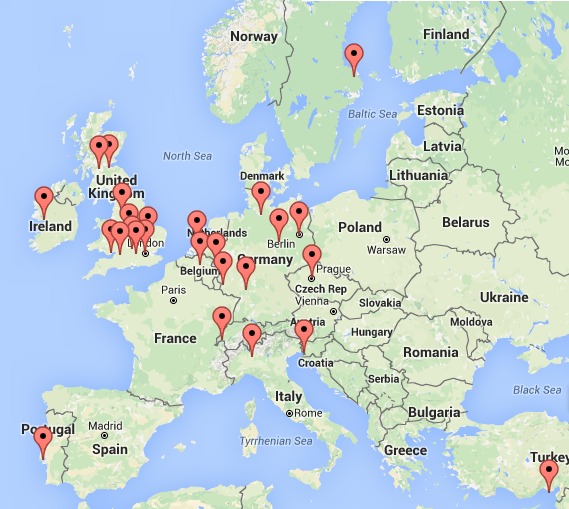
\includegraphics[width=0.9\textwidth]{map}
    The \emph{first} SIAM Student Chapter in the Netherlands is installed at TU Delft.
  \end{center}

\end{textbox}




\begin{textbox}(about) at ($(contents map.south east)+(0cm,-1cm)$) [below left] <25.4cm>
{Who are we?}

  The Chapter at TU Delft has been founded in 2014. The current board:\\
  \begin{center}
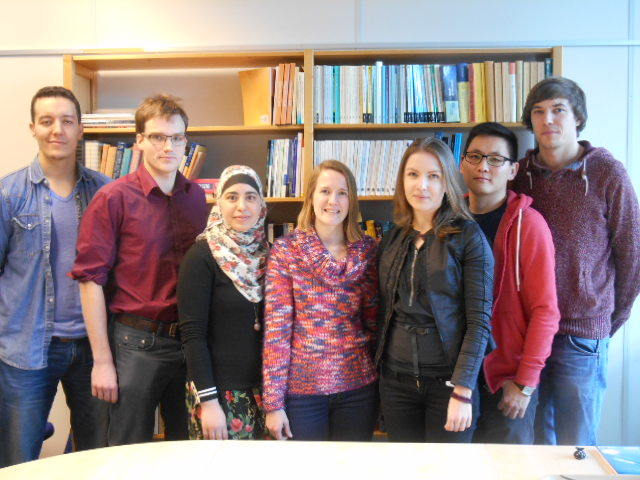
\includegraphics[height=1.4\photobarheight]{board-2015-2016}\\
\end{center}
\bigskip
  The chapter is \emph{open for MSc and PhD students} as well as for staff members.

\end{textbox}

\begin{textbox}(join) at ($(contents about.south east)+(0cm,-1cm)$) [below left] <25.4cm>
{Join us!}

If you wish to join us, please send an email to \emph{SIAMSC-EWI@tudelft.nl} stating your full name and department.

\end{textbox}


\begin{scope}[opacity=0.15,color=black]
  \fill [path fading=south]
    ($(current page.south west)+(-\safetymargin,\footerheight+\photobarbottommargin)$)
    rectangle
    ($(current page.south east)+(\safetymargin,\footerheight+\photobarbottommargin-\photomargin)$);
  \fill
    ($(current page.south west)+(-\safetymargin,\footerheight+\photobarbottommargin)$)
    rectangle
    ($(current page.south east)+(\safetymargin,\footerheight+\photobarbottommargin+\photobarheight-\photomargin)$);
  \fill [path fading=north]
    ($(current page.south west)+(-\safetymargin,\footerheight+\photobarbottommargin+\photobarheight-\photomargin)$)
    rectangle
    ($(current page.south east)+(\safetymargin,\footerheight+\photobarbottommargin+\photobarheight)$);
\end{scope}
\node[above,inner sep=0pt] at ($(current page.south)+(0pt,\footerheight+\photobarbottommargin)$) {%
  \includegraphics[height=\photobarheight]{farm_golf}%
  \hspace{\photomargin}%
  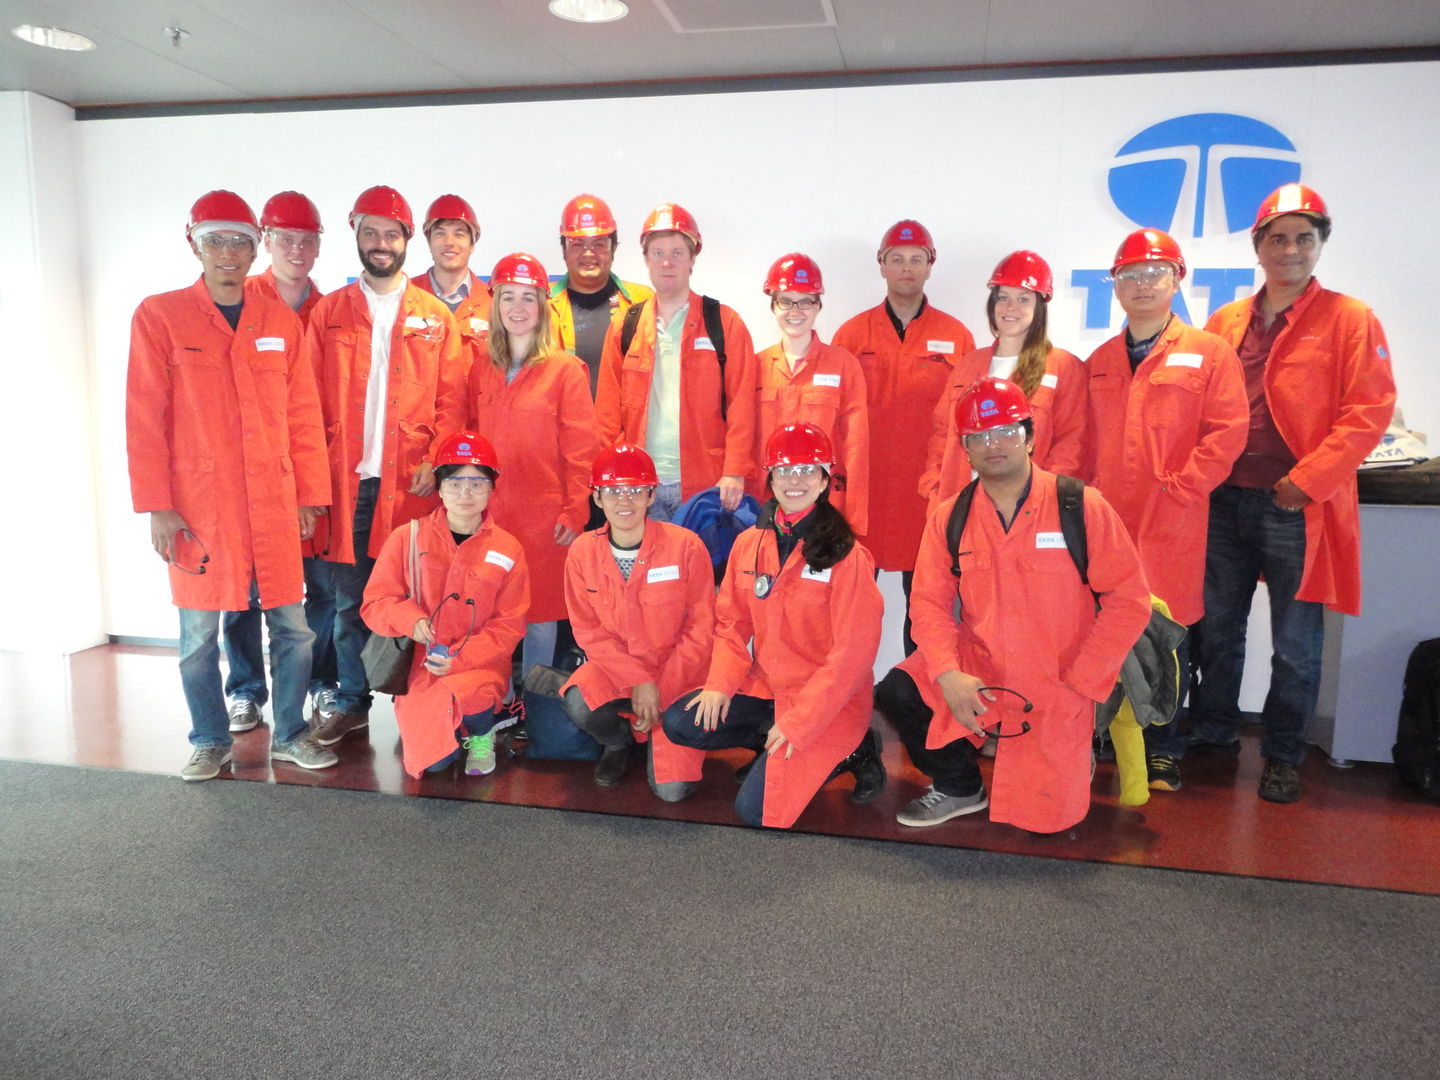
\includegraphics[height=\photobarheight]{tata_group}%
  \hspace{\photomargin}%
  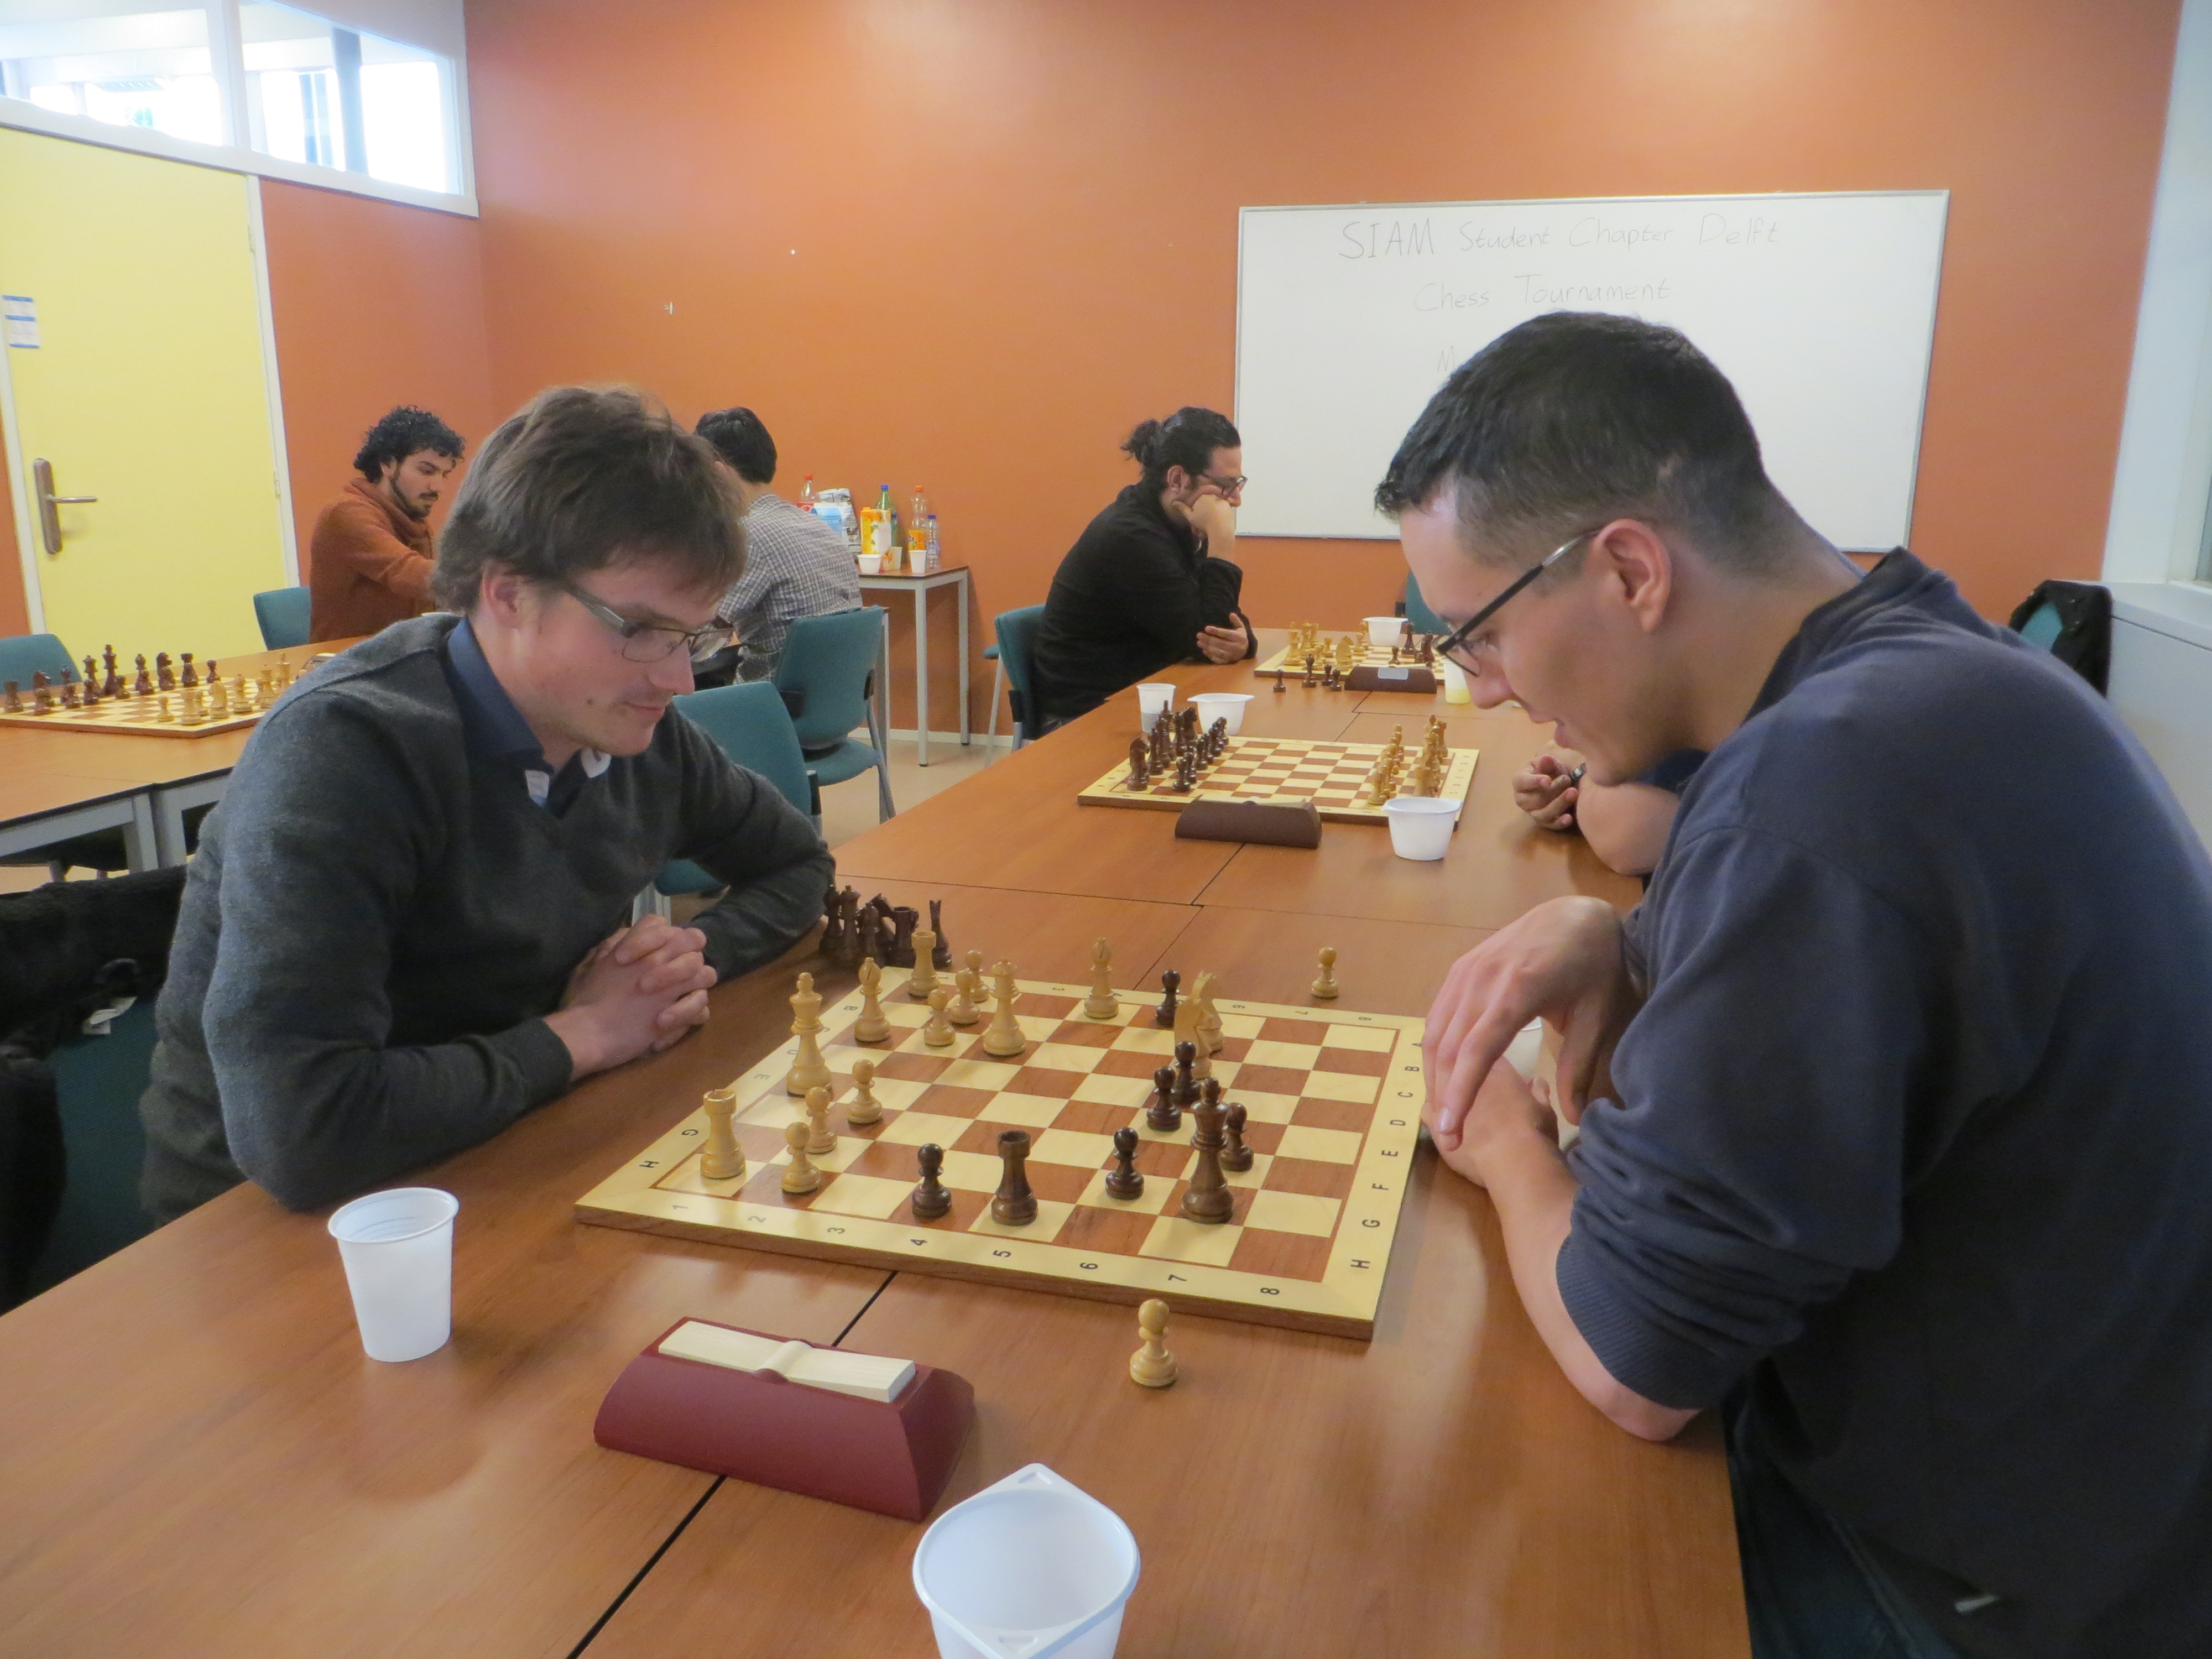
\includegraphics[height=\photobarheight]{chess}%
  \hspace{\photomargin}%
  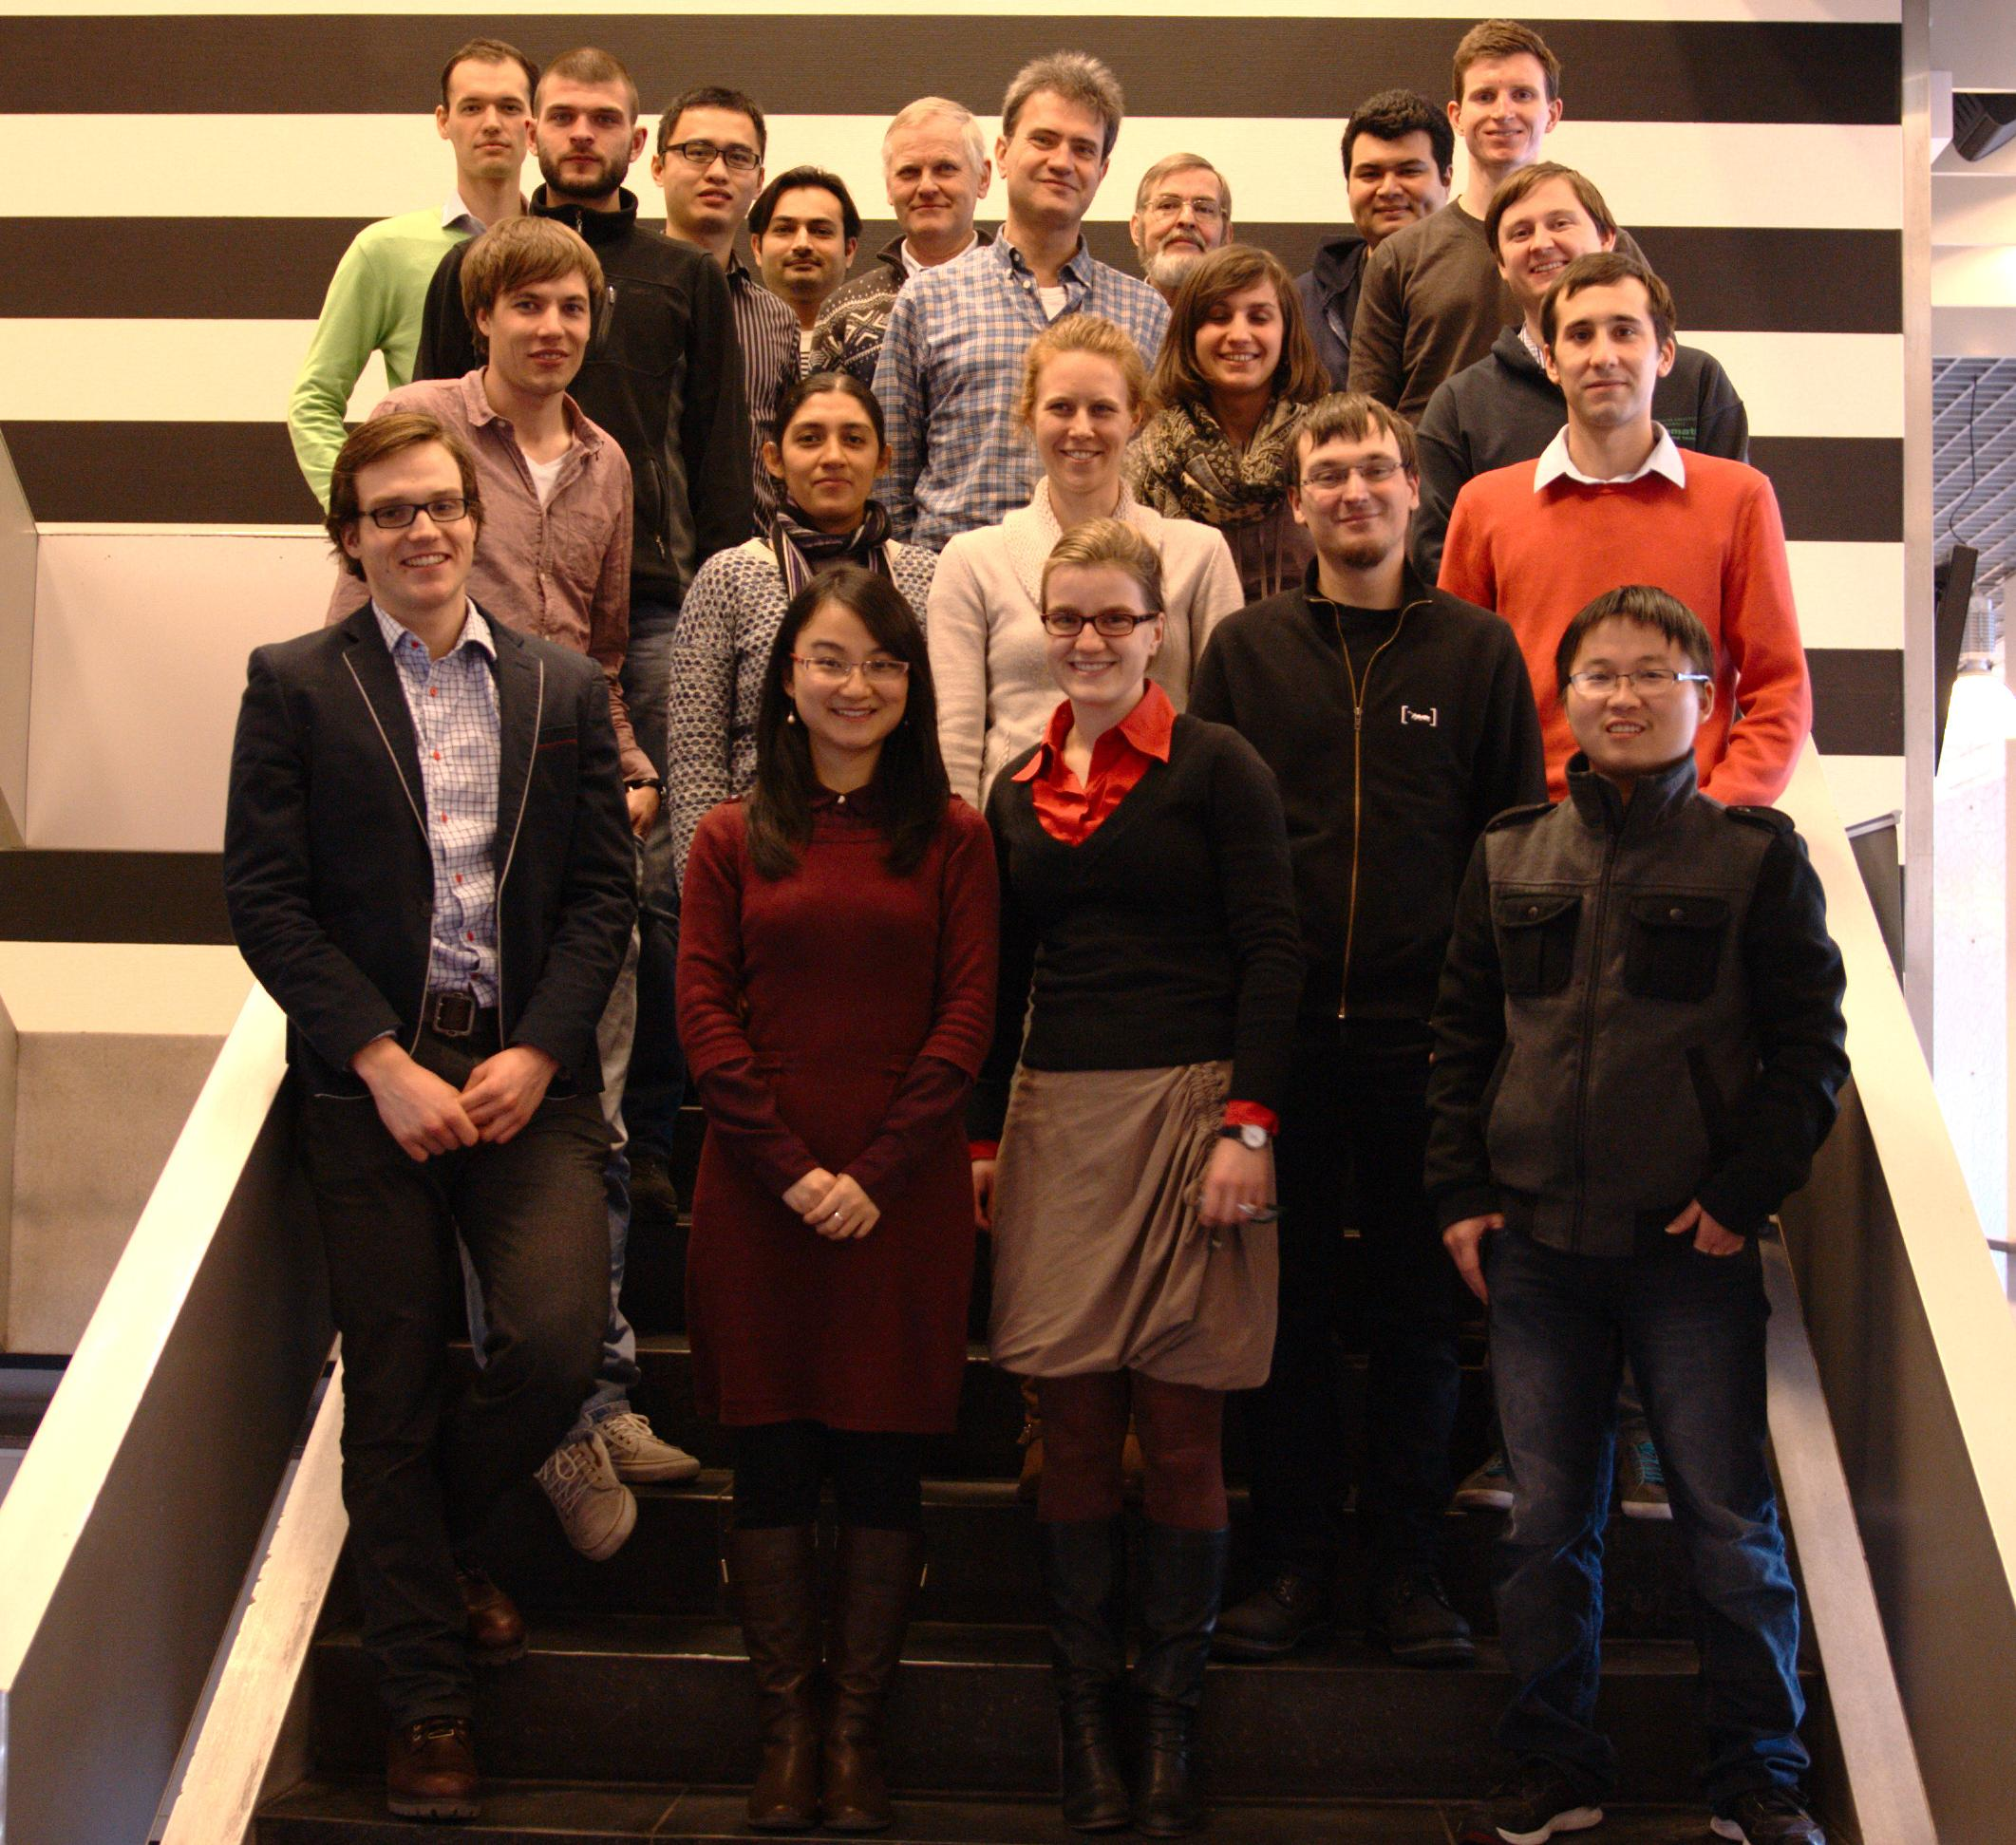
\includegraphics[height=\photobarheight]{KD15_group}%
  \hspace{\photomargin}%
  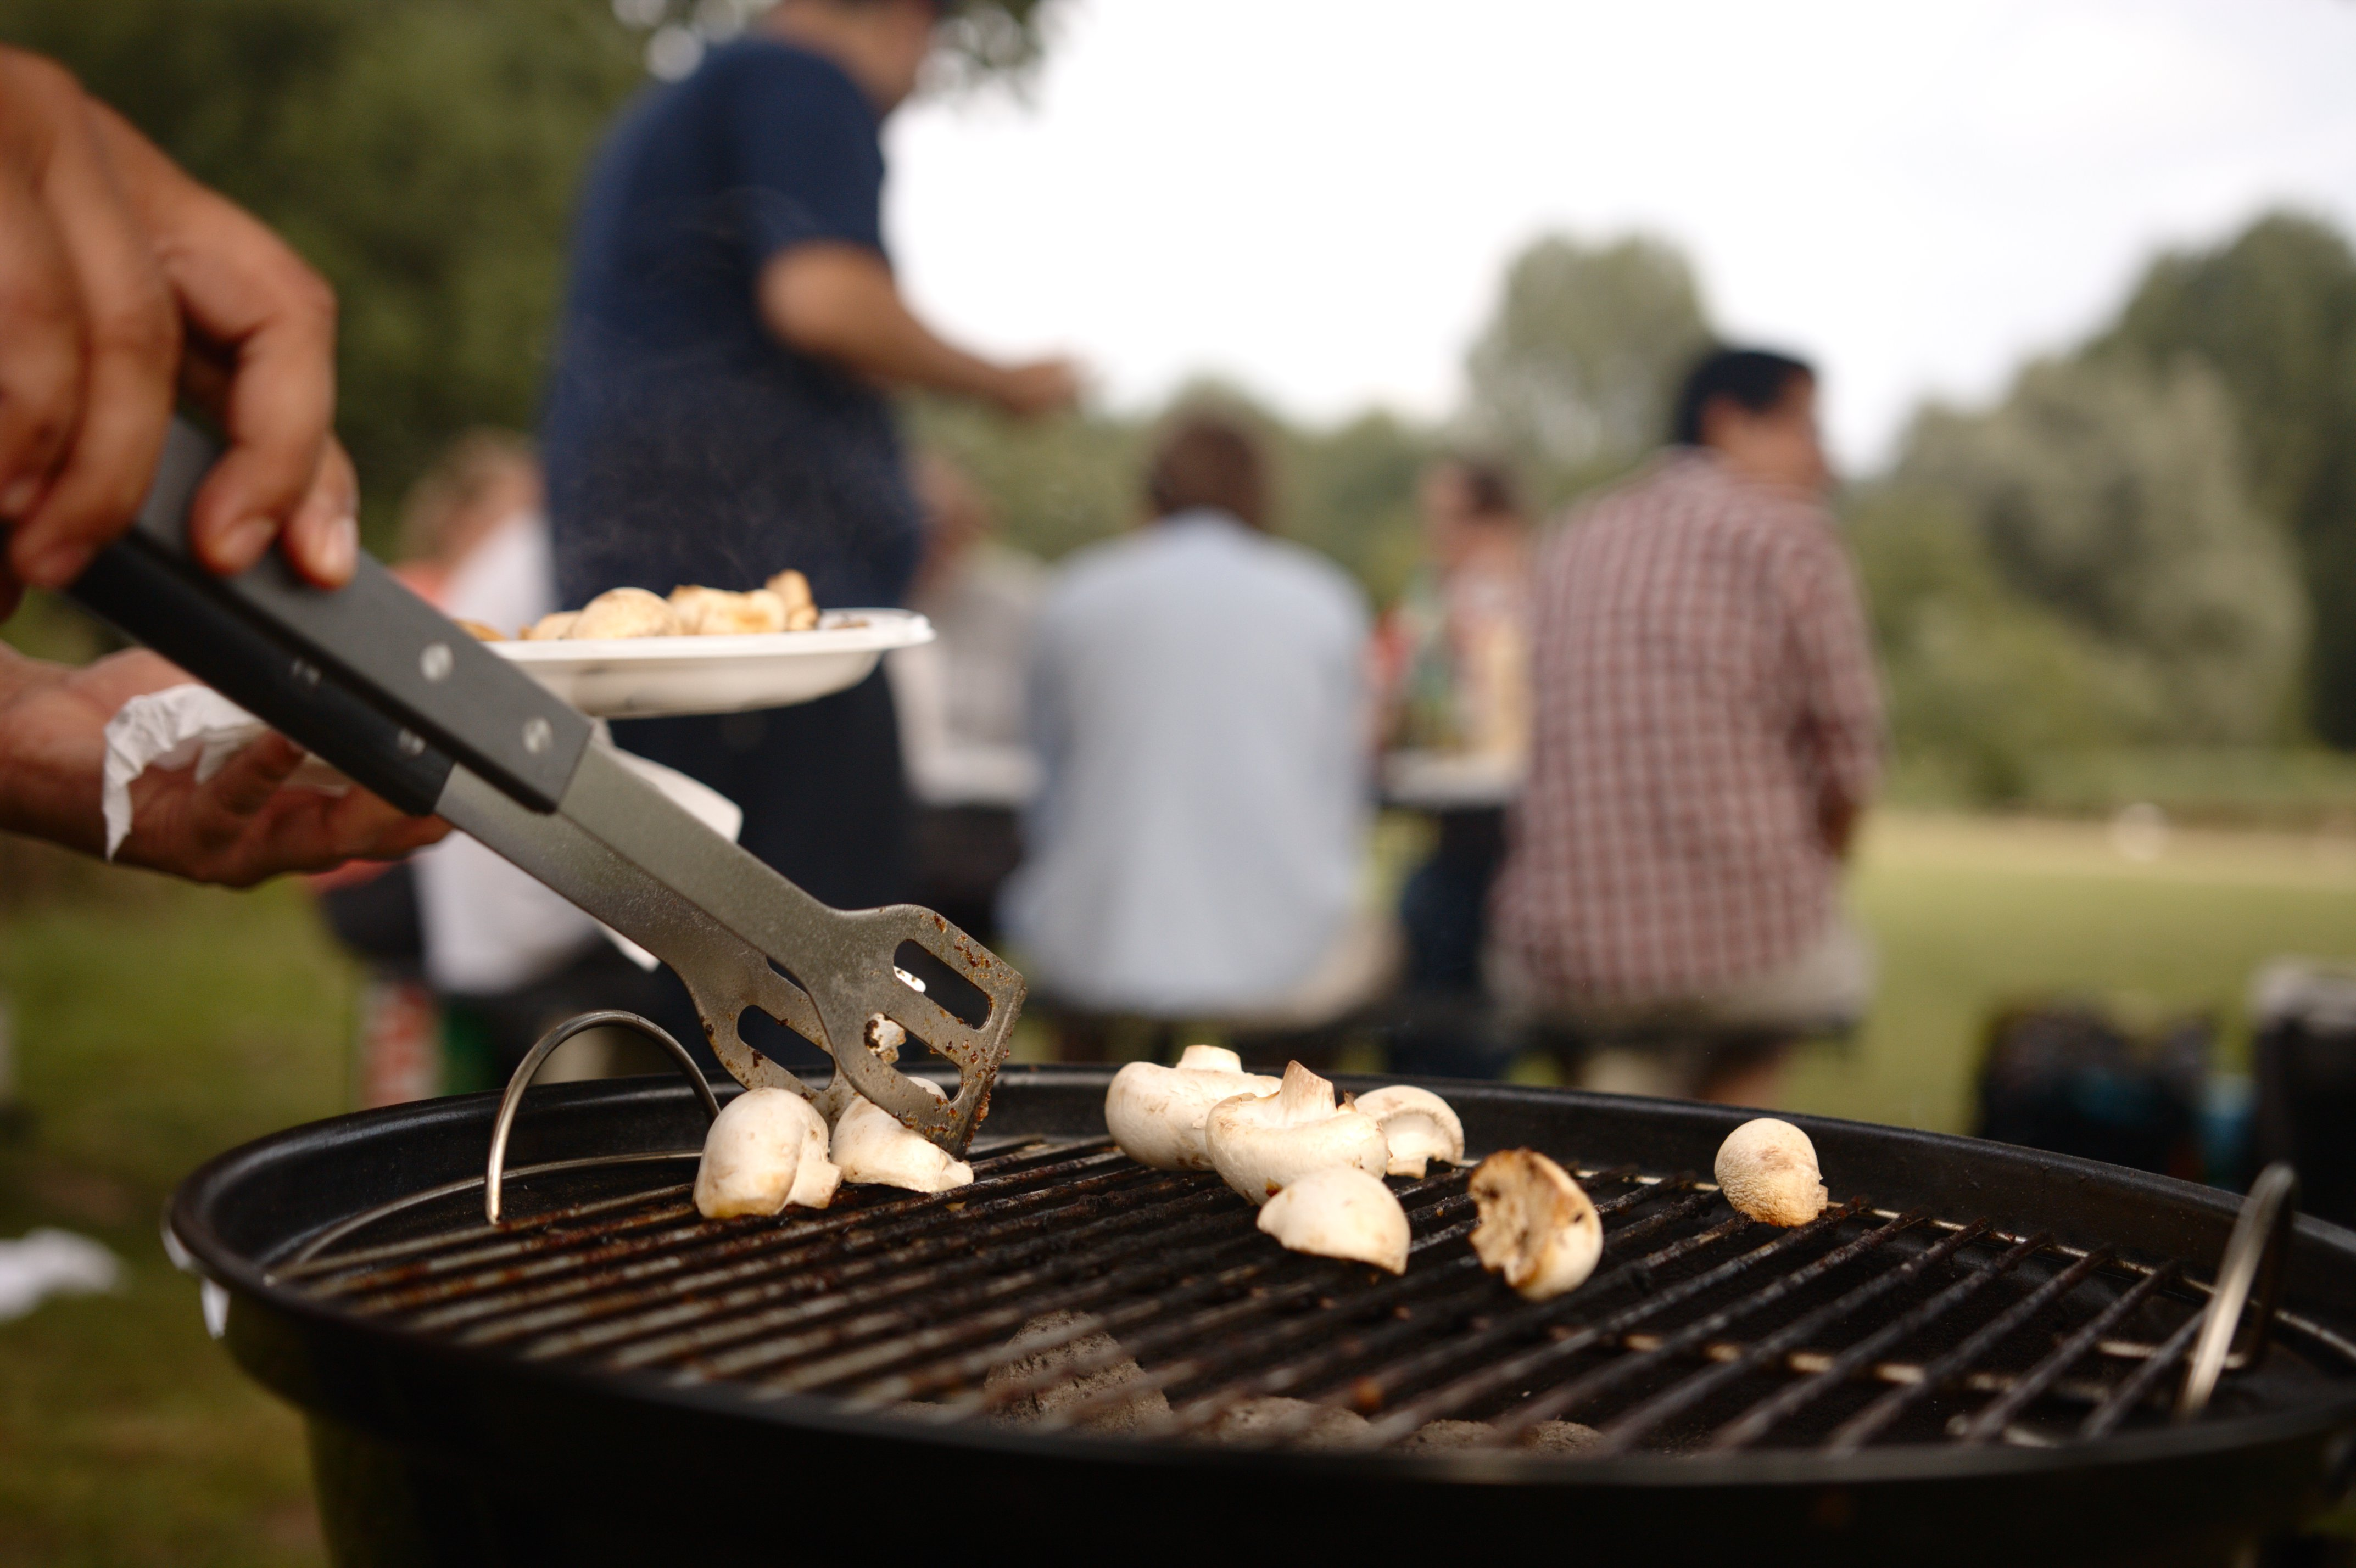
\includegraphics[height=\photobarheight]{bbq2}%
};

\end{tikzpicture}%
\end{document}

% vim: ts=2:sts=2:sw=2:et
